\clearpage
\section{Processi primari}
\label{sec:proc_prim}
\subsection{Fornitura}
\label{sec:fornitura}
Verranno ora trattate le norme che i membri di duckware devono rispettare per poter diventare fornitori nei confronti di \emph{Zero12} e dei committenti, \emph{Prof. Tullio Vardanega} e \emph{Prof. Riccardo Cardin}.
\subsubsection{Ricerca sulle tecnologie}
Questa attività consiste nella ricerca d'informazioni su \markg{framework}, librerie e tutte quelle tecnologie software ritenute utili in una o più fasi di sviluppo del progetto. Il periodo di ricerca è propedeutico a molte attività, in particolare quelle di \emph{Normazione}, \emph{Pianificazione della qualità} e la maggior parte delle attività nel \markg{processo} di sviluppo descritto nella sezione seguente. Viene inclusa anche l'auto-formazione sulle tecnologie scelte.
\subsubsection{Normazione} 
L'amministratore apporta modifiche all'insieme di regole che ciascun membro del team \emph{duckware} deve rispettare durante lo svolgimento dei compiti a lui assegnati. Nel periodo di realizzazione del progetto si riscontrano problemi o si acquisiscono nuove conoscenze che richiedono la modifica delle regole. Un esempio di cambiamento di regole potrebbe essere l'utilizzo di un nuovo strumento ritenuto più appropriato di un altro oppure potrebbero emergere nuovi argomenti per i quali stabilire nuove norme.
\subsubsection{Studio di Fattibilità}
Gli analisti conducono un approfondimento dei \markg{requisiti} per ogni capitolato presentato dai committenti con lo scopo di scegliere se accettare o meno il contratto. In particolare per ciascuna proposta vengono estratte le seguenti informazioni:
\begin{itemize}
	\item Scopo del prodotto da realizzare;
	\item Lista delle tecnologie richieste dal capitolato per realizzare il progetto;
	\item Livello di gradimento verso l'obiettivo del capitolato.
\end{itemize}
\subsubsection{Preparazione alla revisione}
Questa attività consiste nell'approntamento del materiale da presentare in ingresso alla revisione ed eventualmente la preparazione del materiale per l'esposizione, quando prevista. La prima fase comprende anche la scrittura di una lettera di presentazione da parte del \markg{responsabile} di \emph{duckware}.
\subsection{Sviluppo}
\label{sec:sviluppo}
\subsubsection{Analisi dei Requisiti}
L’analisi dei requisiti ha lo scopo di individuare i requisiti richiesti dal capitolato preso in questione. Tali informazioni possono essere reperite da verbali, casi d’uso oppure dai capitolati d’appalto stessi. Il risultato finale di questa analisi porterà alla creazione da parte degli analisti del documento \emph{Analisi dei requisiti v4.0.0} che fornirà informazioni riguardo:
\begin{itemize}
	\item Descrivere l’obiettivo del lavoro del gruppo e fornire riferimenti precisi ai progettisti;
	\item Fornire una lista dettagliata di funzionalità e requisiti concordati col  cliente;
	\item Fornire degli esempi di dialoghi tra l'utente e l'assistente vocale, riferiti alle funzionalità che necessitano di un'interazione tra i due;
	\item Dare ai verificatori riferimenti e casi d’uso per poter creare ed eseguire dei test mirati ed affidabili;
	\item Rendere più semplice il \markg{processo} di revisione del codice.
\end{itemize}
\subsubsection{Classificazione dei Requisiti}
Ogni requisito è identificato da un codice che verrà rappresentato secondo quanto segue:
\begin{center}
	R.{x}.{y}.{z}
\end{center}
\begin{itemize}
	\item \textbf{R}: sta per Requisito;
	\item \textbf{x}: indica l’importanza di tale requisito che può essere 0 (opzionale), 1 (requisito non necessario ma può dare maggiore completezza e definizione) e 2 (obbligatorio in quanto necessario per il funzionamento basilare);
	\item \textbf{y}: assume valore F se requisito funzionale, Q se di qualità, V se di vincolo e P se presentazionale.
	\item \textbf{z}: indica un numero progressivo.
\end{itemize}
\subsubsection{Classificazione dei casi d'uso}
Gli analisti avranno anche cura di identificare i casi d’uso i quali verranno descritti secondo il seguente schema:
\begin{center}
	\textbf{UC[Codice principale].[Codice secondario].[Codice terziario][Codice quaternario] – Identificativo}
\end{center}
\begin{itemize}
	\item \textbf{UC} e \textbf{Identificativo}: Ogni \markg{caso d’uso} è specificato da una serie di cifre spaziate da un punto. Questa serie di cifre identifica una gerarchia, dove il codice principale ha il grado più alto, mentre le altre hanno grado via via più basso. Un trattino separerà il tutto dal nome univoco del caso d’uso;
	\item \textbf{Attori}: gli attori principali e secondari dell’UC (use case);
	\item \textbf{Scopo} e \textbf{descrizione}: una descrizione riassuntiva del caso d’uso;
	\item \textbf{Scenario principale}: usando una lista numerata indica il flusso degli eventi specificando per ognuno a quale caso d’uso si riferisce;
	\item \textbf{Voice flow}: descrive l'eventuale interazione vocale tra l'utente e l'assistente Alexa;
	\item \textbf{Estensioni}: contiene una lista degli eventuali errori che il caso d'uso può generare;
	\item \textbf{Pre-condizione}: specifica le condizioni vere prima del verificarsi degli eventi del caso d’uso;
	\item \textbf{Post-condizione}: specifica le condizioni vere dopo il verificarsi degli eventi del caso d’uso.
\end{itemize}
\subsection{Progettazione}
\label{sec:progettazione}
\subsubsection{Scopo}
La progettazione ha il compito di disegnare, attraverso i Progettisti, una soluzione del problema che sia esaustiva per tutti gli \markg{stakeholders}. Verrà definita la logica del prodotto identificando i componenti e cercando sempre di restare nei costi che sono stati prefissati. In particolare la logica definita dovrà:
\begin{itemize}
	\item Soddisfare i requisiti dell’\emph{Analisi dei requisiti} ed adattarsi ai cambiamenti od alle evoluzioni che potenzialmente avverranno nel tempo;
	\item Essere comprensibile e modulare;
	\item Avere la capacità di rispettare le specifiche nel tempo, anche nel caso di malfunzionamenti;
	\item Ridurre al minimo i tempi di manutenzione;
	\item Le varie parti dovranno poter essere usate anche in altre applicazioni;
	\item Avere un'elevata capacità di rispettare le specifiche nel tempo;
	\item Garantire l'integrità evitando intrusioni da parte di terzi non autorizzati e malfunzionamenti;
	\item Le varie parti devono essere poco dipendenti l'una dalle altre, di modo da poter essere facilmente manutenibili;
	\item Ridurre al minimo i tempi di manutenzione.
\end{itemize}
\subsubsection{Obiettivi}
Essa serve a garantire che il prodotto possa soddisfare le proprietà specificate nell'attività di analisi ponendo i seguenti obiettivi:
\begin{itemize}
    \item Rendere chiara e comprensibile ogni parte dell'\markg{architettura} ai differenti stakeholders;
    \item Garantire la qualità di prodotto sviluppato con lo scopo di raggiungere la \textit{correttezza per costruzione};
    \item Mantenere nascosti i dettagli implementativi secondo quanto espresso dal principio dell'\textit{information hiding};
    \item Mantenere un basso grado di dipendenza fra le varie parti del prodotto;
    \item Ottimizzare l'uso di risorse.
\end{itemize}
\subsubsection{Diagrammi}
Le scelte adottate dai progettisti verranno adeguatamente descritte attraverso l’uso di diagrammi \markg{UML 2.0} per rendere più chiare e meno ambigue le decisioni prese. Verranno in particolare utilizzate le seguenti rappresentazioni:
\begin{itemize}
	\item \textbf{Diagrammi di casi d’uso}: descrivono le funzioni del sistema;
	\item \textbf{Diagrammi delle classi}: descrivono gli oggetti e le dipendenze fra essi;
	\item \textbf{Diagrammi dei package}: descrivono la dipendenza tra i \markg{package} (i quali contengono le classi);
	\item \textbf{Diagrammi di sequenza}: descrivono la collaborazione nel tempo degli oggetti;
	\item \textbf{Diagrammi di attività}: descrivono la logica procedurale.
\end{itemize}
Per poter svolgere nel miglior modo possibile il \markg{processo} di progettazione, il team \textit{duckware} ha deciso di utilizzare il software PlantUML\footnote{\href{http://plantuml.com/}{http://plantuml.com/}}. Quest'ultimo consente di realizzare in maniera semplice e veloce diagrammi delle classi, di attività e di sequenza.
\paragraph{Diagrammi delle classi}\mbox{}\\[0.4cm]
Un diagramma di classe è un grafo orientato che descrive, dal punto di vista statico, l'architettura dell'applicazione mettendo in risalto le relazioni esistenti tra le classi e le interfacce coinvolte nel sistema. Il suo scopo può essere sintetizzato in:
\begin{itemize}
    \item Descrizione delle responsabilità di un sistema;
    \item Base per diagrammi dei componenti e di rilascio;
    \item Analisi e progettazione della visione statica di un'applicazione.
\end{itemize}
Per creare questo tipo di diagrammi in modo semplice, deve essere creato un file per ogni classe, o gruppo di classi, che abbia estensione di tipo \textit{.iuml}. Per stabilire le relazioni presenti tra le varie componenti interessate verrà creato un altro file con estensione \textit{.puml} in modo da avere un diagramma completo. Nel caso in cui una classe non dovesse avere metodi e/o variabili dovrà comunque apparire all'interno del diagramma. I diagrammi delle classi sono collegati fra loro con frecce che evidenziano le dipendenze; in particolare, verranno usati i seguenti tipi di frecce:
\begin{itemize}
    \item \textbf{Freccia semplice}, da A verso B. Indica che la classe A ha una o più istanze di B tra i suoi campi dati;
    \begin{figure}[H]
    	\begin{center}
	    	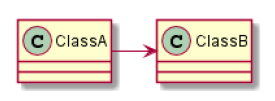
\includegraphics[width=0.55\textwidth]{../includes/pics/frecciasemplice.png}
	    	\caption{Immagine freccia semplice}
	    \end{center}
    \end{figure}
    \item \textbf{Freccia tratteggiata}, da A verso B. Indica che la classe A ha una dipendenza da B secondo una primitiva che andrà specificata vicino alla freccia;
    \begin{figure}[H]
    	\begin{center}
	    	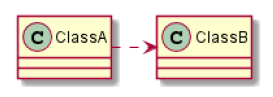
\includegraphics[width=0.55\textwidth]{../includes/pics/frecciatratteggiata.png}
	    	\caption{Immagine freccia tratteggiata}
    	\end{center}
   	\end{figure}
    \item \textbf{Freccia a rombo pieno}, da A verso B. Indica una composizione, una relazione nella quale le classi parte hanno significato solo se legate alla classe tutto;
    \begin{figure}[H]
    	\begin{center}
	    	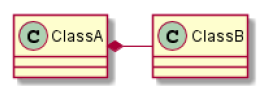
\includegraphics[width=0.55\textwidth]{../includes/pics/frecciarombopieno.png}
	    	\caption{Immagine freccia a rombo pieno}
    	\end{center}
   	\end{figure}
    \item \textbf{Freccia vuota}, da A verso B. Indica il massimo grado di dipendenza fra le classi in quanto stabilisce un rapporto di ereditarietà. Ogni oggetto di A è anche un oggetto di B;
    \begin{figure}[H]
    	\begin{center}
	    	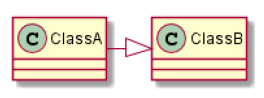
\includegraphics[width=0.55\textwidth]{../includes/pics/frecciavuota.png}
	    	\caption{Immagine freccia vuota}
    	\end{center}
   	\end{figure}
\end{itemize}
%\subsubsection{Diagramma dei package}
\paragraph{Diagrammi dei package}\mbox{}\\[0.4cm]
Ogni package sarà rappresentato da un rettangolo con un'etichetta contenente il relativo nome. All'interno di quest'area ci saranno tutti i diagrammi delle classi appartenenti al package ed eventuali sotto-package. Una dipendenza tra package si indica con una freccia tratteggiata come mostrato nella figura sottostante.
\begin{figure}[H]
	\begin{center}
		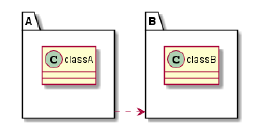
\includegraphics[width=0.55\textwidth]{../includes/pics/packagefreccia.png}
		\caption{Immagine freccia package}
	\end{center}
\end{figure}
%\subsubsection{Diagrammi di sequenza}
\paragraph{Diagrammi di sequenza}\mbox{}\\[0.4cm]
I diagrammi di sequenza vanno letti dall'alto verso il basso in quanto tale senso di lettura indica lo scorrere del tempo. Gli oggetti sono rappresentati con dei rettangoli contenenti un nome per identificarli. Sotto ad ogni istanza ci sarà una linea della vita tratteggiata, che sarà sormontata in alcuni tratti da una barra di attivazione (la quale indica i momenti un cui l'oggetto è attivo). Dalle barre di attivazione partiranno frecce rappresentanti il messaggio/segnale verso la linea di vita di oggetti già istanziati o verso una nuova classe. I tipi di frecce sono i seguenti:
\begin{itemize}
    \item \textbf{Freccia piena}: per indicare un messaggio sincrono e corrisponde alla chiamata di un metodo;
    \item \textbf{Freccia}: per indicare un messaggio asincrono che dunque ritorna immediatamente;
    \item \textbf{Freccia tratteggiata}: per indicare il ritorno di un metodo chiamato e sopra tale freccia andrà indicato il tipo di ritorno;
    \item \textbf{Freccia tratteggiata con create}: per indicare la creazione di un nuovo oggetto;
    \item \textbf{Freccia piena con destroy}: per indicare la distruzione di un oggetto e termina sempre in una \textit{X};
    \item \textbf{Freccia piena}: per indicare un messaggio sincrono e corrisponde alla chiamata di un metodo.
\end{itemize}
\paragraph{Diagrammi di attività}\mbox{}\\[0.4cm]
I diagrammi di attività descrivono il flusso delle attività del software in modo da esplicarne il funzionamento dinamico. Ogni attività viene inserita calcolando che non ci possano essere interferenze durante la sua esecuzione. Un'attività elementare è formata da un nodo iniziale, punto da cui inizia l'esecuzione detto \textit{token}, e da un'activity, contenente la descrizione del token.
\begin{figure}[H]
	\begin{center}
		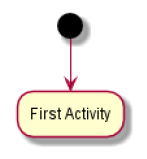
\includegraphics[width=0.55\textwidth]{../includes/pics/attivitabase.png}
		\caption{Immagine freccia attività}
	\end{center}
\end{figure}
Il token è rappresentato da un pallino pieno, l'activity è un rettangolo con del testo all'interno contenente la descrizione che dovrà essere molto sintetica. Vi sono anche altre componenti che possono far parte di un diagramma di attività:
\begin{itemize}
    \item \textbf{Subactivity}: rappresentata da un rettangolo con il nome all'interno ed un piccolo tridente in basso a destra. Ciascuna sotto attività ha un input ed un output;
    \item \textbf{Branch}: rappresentato da un rombo con una freccia in ingresso ed \textit{n} frecce in uscita. Si può prendere solo uno dei rami e ciascuno di questi deve avere scritta la guardia. Consuma e produce token;
    \item \textbf{Merge}: rappresentato da un rombo con \textit{n} frecce in ingresso ed una in uscita. Esso è il punto in cui gli \textit{n} rami di un \markg{branch} tornano ad unirsi. Consuma e produce token;
    \item \textbf{Fork}: rappresentato da una linea lunga orizzontale o verticale, è il punto il cui l'attività si parallelizza senza vincoli temporali di esecuzione. Consuma un token e ne genera \textit{n};
    \item \textbf{Join}: rappresentato da una linea lunga orizzontale o verticale, è il punto in cui avviene la sincronizzazione fra processi paralleli. Consuma \textit{n} token e ne genera uno;
    \item \textbf{Segnali}: rappresentati da due figure ad incastro con la prima non bloccante emette il segnale mentre la seconda è bloccante e riceve il segnale;
    \item \textbf{Timeout}: rappresentato da una clessidra, serve a modellare il timeout o eventi ripetuti. Hanno frecce entranti ed uscenti. Un timeout deve cominciare con la descrizione \textit{wait} mentre un ciclo ripetuto con \textit{every};
    \item \textbf{Nodo fine flusso}: rappresentato da un cerchio vuoto con una X al centro, è il punto in cui un ramo di esecuzione muore;
    \item \textbf{Nodo finale}: rappresentato da due cerchi concentrici, è il punto in cui termina l'esecuzione e consuma un token.
\end{itemize}
\subsubsection{Sviluppo}
Lo sviluppo del progetto avviene seguendo il modello iterativo secondo quando spiegato nel documento \textit{Piano di progetto}. Il team \textit{duckware} ha deciso di utilizzare le tecnologie specificate dalla proponente in quanto ha ritenuto che siano adatte per la realizzazione del prodotto e che non ne siano necessarie ulteriori. Il \markg{capitolato d'appalto} consiglia le seguenti tecnologie:
\begin{itemize}
    \item \textbf{Java}: per lo sviluppo dell'applicazione e la comunicazione di essa con i servizi di AWS;
    \item \textbf{Node.js}: per l'integrazione di Alexa con l'infrastruttura di AWS;
    \item \textbf{AWS}: servizi di Amazon per la realizzazione del database delle API; nel particolare verranno utilizzati: 
    \begin{itemize}
        \item \textbf{AWS DynamoDB}: per la gestione dei dati;
        \item \textbf{AWS Lambda}: per l'implementazione del servizio \markg{serverless}.
    \end{itemize}
\end{itemize}
\subsubsection{Obiettivi della progettazione}
La progettazione garantisce che il prodotto finale soddisfi tutte le richieste emerse e specificate durante l’analisi. Deve garantire la qualità del prodotto sviluppato e cercare di ottimizzare l’uso delle risorse disponibili. Inoltre, una buona progettazione cerca di suddividere nel migliore dei modi i compiti implementativi al fine di ridurre la complessità del problema e, di conseguenza, facilitare il compito dei programmatori.
\subsection{Codifica}
\label{sec:codifica}
I programmatori dovranno rispettare alcune regole che garantiranno uniformità e coesione al codice che verrà prodotto durante la creazione del progetto. Ci sono sia delle norme globali alle quali i programmatori si devono attenere, indipendentemente dal linguaggio di programmazione scelto, sia delle norme specifiche legate a Java e Node.js.\\[0.5cm]
Per chiarezza ogni norma avrà un suo paragrafo composto di titolo, descrizione ed esempio illustrativo di quanto si vuole specificare.\\[0.5cm]
\textbf{Convenzioni per i nomi}
\begin{itemize}
	\item Ogni nome deve essere unico e soprattutto deve essere appropriato, ovvero deve descrivere al meglio ciò che rappresenta;
	\item In caso di nome formato dalla composizione di più parole, si potrà utilizzare l’underscore come separatore. In alternativa, si potranno separare i termini con una lettera maiuscola secondo la modalità detta \markg{lowerCamelCase}. Ad esempio:
	\begin{itemize}
		\item \texttt{variable\char`_name}
		\item \texttt{ANOTHER\char`_EXAMPLE\char`_FOR\char`_THIS}
		\item \texttt{yetAnotherExample}
	\end{itemize}
	\item Usare le lettere maiuscole quando si intende utilizzare una parola come attributo \emph{const} (costante). Altrimenti, usare lettere minuscole. Per esempio:
	\begin{itemize}
		\item \emph{(costante)} \texttt{variable\char`_name}
		\item (\textbf{non} costante) \texttt{ANOTHER\char`_EXAMPLE\char`_FOR\char`_THIS}
		\item (\textbf{non} costante) \texttt{yetAnotherExample}
	\end{itemize}
\end{itemize}
\textbf{Convenzioni per la documentazione}
\begin{itemize}
	\item I commenti ed i nomi presenti nel documento devono tassativamente essere scritti in inglese;
	\item Ogni file dovrà contenere nella sua intestazione, come commento, la seguente struttura:
\begin{table} [H]
	\begin{center}
		\begin{tabular}{| l |}
			\hline
			File : filename.java\\
			Version : versione file\\
			Date : data di creazione\\
			Author : nome autore/i\\
			\\
			License : tipo di licenza del file\\
			\\
			Changelog : Autore || Data || breve descrizione delle modifiche\\
			\hline
		\end{tabular}
	\end{center}
	\caption{Esempio commento intestazione file}
\end{table}
\end{itemize}

%\begin{figure} [h]
%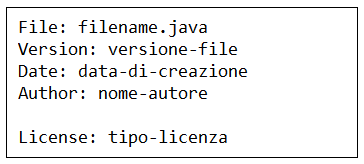
\includegraphics[width=1\textwidth]{../includes/pics/foto2_4.png}
%\caption{Esempio convenzioni per la documentazione}
%\end{figure}
\begin{itemize}
	\item La versione va inserita come X.Y dove:
	\begin{itemize}
		\item \textbf{X}: indica la versione principale ed è da incrementare \textbf{solo ed esclusivamente} nel caso in cui si passi ad una versione stabile. Un tale incremento comporta l’azzeramento di Y;
		\item \textbf{Y}: indica la versione parziale ed un incremento di tale indice rappresenta una verifica o una modifica rilevante che verrà sottoposta alla fase di test.
	\end{itemize}
\end{itemize}
\subsubsection{Java}
In questa sezione vengono indicate delle convenzioni adottate dal team di 
\markg{\href{https://google.github.io/styleguide/javaguide.html}{Google}} che dovranno essere rispettate nel progetto dagli sviluppatori durante la scrittura del codice.
\paragraph{Commenti}\mbox{}\\[0.4cm]
I commenti su singola riga possono essere inseriti tramite l’uso di un doppio slash \emph{(single line comment block)} oppure da uno slash seguito da un asterisco \emph{(multi-line comment block)}. Quest’ultima tecnica deve essere utilizzata anche per i commenti su più righe dove, per ciascun inizio di riga, deve essere presente un asterisco. È necessario inserire uno spazio dopo ogni asterisco di inizio riga, se presente.
\begin{table} [H]
	\begin{center}
		\begin{tabular}{ | l | l |}
			\multicolumn{1}{c}{\textbf{OK}}&\multicolumn{1}{c}{\textbf{NO}}\\ 
			\hline
			//commento su singola riga & //commento\\
			& //su più\\
			/* commento su singola riga */& //righe\\
			&\\
			/* commento&/*commento\\
			\hspace{0.2cm}* su più&\hspace{0.2cm}*su più\\
			\hspace{0.2cm}* righe */&\hspace{0.2cm}*righe*/\\
			\hline
		\end{tabular}
	\end{center}
	\caption{Esempio commenti}
\end{table}
Ogni file \texttt{.java} dovrà contenere in testa un commento a singola o multipla riga che descriva brevemente il contenuto del file e le funzionalità che offre.
\paragraph{Indentazione}\mbox{}\\[0.4cm]
Il corpo di ogni funzione dovrà essere separato dall’inizio della riga con una tabulazione, lasciando le impostazioni standard fornite dall’IDE. In caso di istruzioni di controllo annidate, ognuna dovrà essere propriamente incolonnata e spaziata da tabulazioni rispetto all'inizio della riga.
\begin{table} [H]
	\begin{center}
		\begin{tabular}{ | l | l |}
			\multicolumn{1}{c}{\textbf{OK}}&\multicolumn{1}{c}{\textbf{NO}}\\ 
			\hline
			double test(int a) \{ & double test(int a) \{\\
			\hspace{0.5cm}if (a > 5) \{ 			   &  if (a > 5) \{\\
			\hspace{1cm}return a * 10;          & \hspace{0.5cm}return a * 10;\\
		    \hspace{0.5cm}\} else \{ 					& \} else \{\\
			\hspace{1cm}return a * 20;          & \hspace{0.5cm}return a * 20;\\
			\hspace{0.5cm}\}								& \}\\
			\}								& \}\\
			\hline
		\end{tabular}
	\end{center}
\caption{Esempio indentazione}
\end{table}
\paragraph{Blocchi di inizio e fine}\mbox{}\\[0.4cm]
Ogni blocco dovrà essere contrassegnato dalle parentesi graffe, anche quando esse potrebbero essere omesse, per evitare problemi di comprensione del codice. Nello specifico:
\begin{table} [H]
	\begin{center}
		\begin{tabular}{ | l | l |}
			\multicolumn{1}{c}{\textbf{OK}}&\multicolumn{1}{c}{\textbf{NO}}\\ 
			\hline
			if (true) \{ 			   &  if (true)\\
			\hspace{0.5cm}return true;          & \hspace{0.5cm}return true;\\
			\} else \{ 					& else\\
			\hspace{0.5cm}return false;          & \hspace{0.5cm}return false;\\
			\}								& \\
			\hline
		\end{tabular}
	\end{center}
	\caption{Esempio blocchi di inizio e fine}
\end{table}
La stessa regola vale anche nel caso di statements quali \texttt{while, for} e tutti quelli che consentono l’omissione delle parentesi graffe in caso di istruzione singola.
\paragraph{Nomi - Variabili}\mbox{}\\[0.4cm]
I nomi delle variabili vanno sempre scritti con una lettera minuscola iniziale ed il resto del corpo deve essere anch’esso minuscolo. In caso di variabili formate da parole composte, è possibile scrivere alcuni caratteri in maiuscolo:
\begin{table} [H]
		\begin{center}
			\begin{tabular}{ | l | l |}
				\multicolumn{1}{c}{\textbf{OK}}&\multicolumn{1}{c}{\textbf{NO}}\\ 
				\hline
				void test() \{
				&void test() \{\\
				\hspace{0.5cm}int a;
				&\hspace{0.5cm}int A;\\
				\hspace{0.5cm}String qualcosa;
				&\hspace{0.5cm}String Qualcosa;\\
				\hspace{0.5cm}String qualcosaAltro;
				&\hspace{0.5cm}String QualcosaAltro;\\
				\hspace{0.5cm}bool ancoraAltro2;
				&\hspace{0.5cm}bool ANCORAALTRO;\\
				&\}\\
				\hspace{0.5cm}//...									&
				\\
				\}&\\
				\hline
			\end{tabular}
		\end{center}
		\caption{Esempio nomi variabili}
\end{table}
	
La modalità di scrittura delle variabili appena descritto è conosciuto come lowerCamelCase. Sarà anche possibile separare i nomi delle variabili utilizzando un underscore ma, in questo caso, ogni carattere dovrà essere completamente minuscolo o in maiuscolo (e quindi non adottare il lowerCamelCase).\\
\begin{table} [H]
	\begin{center}
		\begin{tabular}{ | l | l |}
			\multicolumn{1}{c}{\textbf{OK}}&\multicolumn{1}{c}{\textbf{NO}}\\ 
			\hline
			void test() \{
			&void test() \{\\
			\hspace{0.5cm}int \_a;
			&\hspace{0.5cm}int \_A;\\
			\hspace{0.5cm}String qualcosa\_altro;
			&\hspace{0.5cm}String QUALCOSA\_altro;\\
			\hspace{0.5cm}String qualcosaAltro;
			&\hspace{0.5cm}String Qualcosa\_Altro;\\
			\hspace{0.5cm}bool QUALCOSA\_ALTRO\_2;
			&\hspace{0.5cm}bool Ancora\_Altro\_2;\\
			&\\
			\hspace{0.5cm}//...									&
			\hspace{0.5cm}//... \\
			\}&\}\\
			\hline
		\end{tabular}
	\end{center}
	\caption{Esempio lowerCamelCase}
\end{table}
	
In caso di costanti, sarà necessario scrivere la variabile in maiuscolo e si potranno anche usare gli underscore.\hspace{1cm}\texttt{PI\_VALUE  = 3.1415;} \hspace{0.5cm} \texttt{PIVALUE = 3.1415;}\\[0.5cm]
È fondamentale e necessario che ogni nome di variabile (comprese quelle costanti) debba avere un significato e rappresentare ciò che quella variabile indica. Non sono quindi ammessi nomi di variabili o costanti quali \texttt{pippo} o \texttt{gigi}.
\paragraph{Nomi - Metodi e procedure}\mbox{}\\[0.4cm]
I nomi dei metodi devono essere scritti rispettando le regole del lowerCamelCase. Solitamente la nomenclatura deve essere relativa ad un verbo o ad una frase come ad esempio \texttt{inviaMessaggio} oppure \texttt{stop}.
\begin{table} [H]
	\begin{center}
		\begin{tabular}{ | l | l |}
			\multicolumn{1}{c}{\textbf{OK}}&\multicolumn{1}{c}{\textbf{NO}}\\ 
			\hline
			void test() \{& void TEST() \{\\
			\hspace{0.5cm} //... & \hspace{0.5cm} //...\\
			\}&\}\\
			&\\
			void testMethod() \{ & void TestMethod() \{ \\
			\hspace{0.5cm} //... & \hspace{0.5cm} //... \\
			\}&\}\\
			\hline
		\end{tabular}
	\end{center}
	\caption{Esempio nomi metodi}
\end{table}
Non è possibile usare gli underscore per separare il nome del metodo in più unità sintattiche. I nomi dei parametri dei metodi devono anch’essi aderire allo stile di scrittura \markg{CamelCase}.
\paragraph{Nomi – Classi ed interfacce}\mbox{}\\[0.4cm]
I nomi delle classi devono essere scritti rispettando le regole dell’\markg{UpperCamelCase}. Tipicamente i nomi delle classi sono nomi o brevi descrizioni come ad esempio \texttt{Character} oppure \texttt{ListaImmutabile}. Le stesse regole si applicano per le interfacce ma queste ultime, in più, possono anche avere un nome che sia un aggettivo come \texttt{Leggibile} (dall’inglese \texttt{Readable}).
\begin{table} [H]
	\begin{center}
		\begin{tabular}{  l | l }
			\multicolumn{1}{c}{\textbf{OK}}&\multicolumn{1}{c}{\textbf{NO}}\\ 
			
			class Dog \{
			& class dog \{ \\
			\hspace{0.5cm}//...
			& \hspace{0.5cm}//... \\
			\}
			& \} \\
			&\\
			class BuildingBlock \{
			& class BUILDING\_BLOCK \{\\
			\hspace{0.5cm}//...
			& \hspace{0.5cm}//...\\
			\}
			&\}\\
			&\\
			interface Drinkable \{
			& interface Drink \{\\
			\hspace{0.5cm}//...
			& \hspace{0.5cm}//...\\
			\}
			& \}\\
			&\\
			class Water implements Drinkable \{
			& class water implements Drink \{ \\
			\hspace{0.5cm}//...									& \hspace{0.5cm}//...\\
			\}
			& \}\\		
		\end{tabular}
	\end{center}
	\caption{Esempio nomi classi}
\end{table}
	
\paragraph{Regole pratiche}\mbox{}\\[0.4cm]
\begin{enumerate}
	\item Quando si fa l’\markg{override} di un metodo è necessario inserire sempre l’annotazione \texttt{@Override}. Nel caso il metodo sia stato marcato con \texttt{@Deprecated}, allora non è necessario inserire l’annotazione di override.
	\begin{table} [H]
		\begin{center}
			\begin{tabular}{ | l | l |}
				\multicolumn{1}{c}{\textbf{OK}}&\multicolumn{1}{c}{\textbf{NO}}\\ 
				\hline
				public Test implements Runnable \{& public Test implements Runnable \{\\
				&\\
				\hspace{0.5cm}@Override & \hspace{0.5cm}public void run() \{ \\
				\hspace{0.5cm}public void run() \{& \hspace{1cm}//...\\
				\hspace{1cm}//... & \hspace{0.5cm}\} \\
				\hspace{0.5cm}\}&\}\\
				\}&\\
				\hline
			\end{tabular}
		\end{center}
		\caption{Esempio regole pratiche}
	\end{table}
		
	\item Nel caso di eccezioni da catturare, queste non devono essere ignorate o catturate senza eseguire alcuna azione. Questa pratica, detta \emph{“exception swallowing”} non è permessa. 
	\begin{table} [H]
		\begin{center}
			\begin{tabular}{ | l | l |}
				\multicolumn{1}{c}{\textbf{OK}}&\multicolumn{1}{c}{\textbf{NO}}\\ 
				\hline
				try \{	& try \{\\
				\hspace{0.5cm} qualcosa(); & \hspace{0.5cm} qualcosa();\\
				\hspace{0.5cm} qualcosaAltro(); & \hspace{0.5cm} qualcosaAltro();\\
			    \} catch (IOException e )\{  & \} catch (IOException e )\{\\
			    \hspace{0.5cm} handle(e); & \}\\
			    \}&\\
	   			\hline
			\end{tabular}
		\end{center}
		\caption{Esempio regole pratiche}
	\end{table}
	Nell’esempio, il metodo \texttt{handle()} è identificativo del fatto che verrà eseguita qualche azione che possa notificare la cattura dell’eccezione.
	\item Scrivere metodi che siano il più corti possibile. Quando si eccedono le 40 righe, conviene considerare la possibilità di spezzare il codice e distribuirlo su più metodi.
	\item Utilizzare commenti TODO a singola linea che descrivano brevemente cosa deve essere ancora implementato nel metodo oppure se ci sono correzioni da fare.  
	
	\begin{flushleft}
	\texttt{// TODO: aggiungere un flag nel ciclo for che indichi lo stato della variabile x}
	\end{flushleft}

\end{enumerate}

\subsubsection{Node.js}
In questa sezione vengono indicate le convenzioni indicate dal team di sviluppo di Node.js\footnote{\href{https://docs.npmjs.com/misc/coding-style.html}{https://docs.npmjs.com/misc/coding-style.html}} che dovranno essere rispettate nel progetto dagli sviluppatori durante la scrittura del codice.
\paragraph{Commenti}\mbox{}\\[0.4cm]
I commenti su singola riga possono essere inseriti tramite l’uso di un doppio slash \emph{(single line comment block)} oppure da uno slash seguito da un asterisco \emph{(multi-line comment block)}. Quest’ultima tecnica deve essere utilizzata anche per i commenti su più righe dove, per ciascun inizio di riga, deve essere presente un asterisco. È necessario inserire uno spazio dopo ogni asterisco di inizio riga, se presente.
\begin{table} [H]
	\begin{center}
		\begin{tabular}{ | l | l |}
			\multicolumn{1}{c}{\textbf{OK}}&\multicolumn{1}{c}{\textbf{NO}}\\ 
			\hline
			//commento su singola riga & //commento\\
			& //su più\\
			/* commento su singola riga */& //righe\\
			&\\
			/* commento&/*commento\\
			\hspace{0.2cm}* su più&\hspace{0.2cm}*su più\\
			\hspace{0.2cm}* righe */&\hspace{0.2cm}*righe*/\\
			\hline
		\end{tabular}
	\end{center}
	\caption{Esempio commenti di Node.js}
\end{table}
Ogni file \texttt{.js} dovrà contenere in testa un commento a singola o multipla riga che descriva brevemente il contenuto del file e le funzionalità che offre.
\paragraph{Indentazione}\mbox{}\\[0.4cm]
Vanno bene le impostazioni di indentazione fornite dell'editor Visual Studio Code per Node.js. Non ci sono restrizioni sull'uso della tabulazione o del doppio spazio, anche se il primo approccio è preferibile.
\paragraph{Blocchi di inizio e fine}\mbox{}\\[0.4cm]
Ogni blocco dovrà essere contrassegnato dalle parentesi graffe, anche quando esse potrebbero essere omesse, per evitare problemi di comprensione del codice. La parentesi graffa di apertura deve stare nella stessa linea del costrutto che inizializza.
\begin{table} [H]
	\begin{center}
		\begin{tabular}{ | l | l |}
			\multicolumn{1}{c}{\textbf{OK}}&\multicolumn{1}{c}{\textbf{NO}}\\ 
			\hline
			if (true) \{ 			   &  if (true)\\
			\hspace{0.5cm}return true;          & \hspace{0.5cm} \{ return true; \}\\
			\} else \{ 					& else\\
			\hspace{0.5cm}return false;          & \hspace{0.5cm}return false;\\
			\}								& \\
			\hline
		\end{tabular}
	\end{center}
	\caption{Esempio blocchi di inizio e fine}
\end{table}
La stessa regola vale anche nel caso di statements quali \texttt{while, for} e tutti quelli che consentono l’omissione delle parentesi graffe in caso di istruzione singola.
\begin{table} [H]
	\begin{center}
		\begin{tabular}{ | l | l |}
			\multicolumn{1}{c}{\textbf{OK}}&\multicolumn{1}{c}{\textbf{NO}}\\ 
			\hline
			if (true) \{ 			   &  if (true) \{ method(); \}\\
			\hspace{0.5cm}method();          &   \\
			\}  					& while (true)\\     
			while(true) \{          & \hspace{0.5cm}method2(); \\
			\hspace{0.5cm}method2();          & \\
			\}								& \\
			\hline
		\end{tabular}
	\end{center}
	\caption{Esempio 2 di blocchi di inizio e fine}
\end{table}
\paragraph{Variabili}\mbox{}\\[0.4cm]
I nomi delle variabili vanno sempre scritti con una lettera minuscola iniziale ed il resto del corpo deve essere anch’esso minuscolo. In caso di variabili formate da parole composte, è possibile scrivere alcuni caratteri in maiuscolo:
\begin{table} [H]
		\begin{center}
			\begin{tabular}{ | l | l |}
				\multicolumn{1}{c}{\textbf{OK}}&\multicolumn{1}{c}{\textbf{NO}}\\ 
				\hline
				void test() \{
				&void test() \{\\
				\hspace{0.5cm}var a;
				&\hspace{0.5cm}var A;\\
				\hspace{0.5cm}var qualcosa;
				&\hspace{0.5cm}var Qualcosa;\\
				\hspace{0.5cm}var qualcosaAltro;
				&\hspace{0.5cm}var QualcosaAltro;\\
				\hspace{0.5cm}var ancoraAltro2;
				&\hspace{0.5cm}var ANCORAALTRO;\\
				&\}\\
				\hspace{0.5cm}//...									&
				\\
				\}&\\
				\hline
			\end{tabular}
		\end{center}
		\caption{Esempio nomi variabili}
\end{table}
	
Sarà anche possibile separare i nomi delle variabili utilizzando un underscore ma, in questo caso, ogni carattere dovrà essere completamente minuscolo o in maiuscolo (e quindi non adottare il lowerCamelCase).\\
\begin{table} [H]
	\begin{center}
		\begin{tabular}{ | l | l |}
			\multicolumn{1}{c}{\textbf{OK}}&\multicolumn{1}{c}{\textbf{NO}}\\ 
			\hline
			void test() \{
			&void test() \{\\
			\hspace{0.5cm}var \_a;
			&\hspace{0.5cm}var \_A;\\
			\hspace{0.5cm}var qualcosa\_altro;
			&\hspace{0.5cm}var QUALCOSA\_altro;\\
			\hspace{0.5cm}var qualcosaAltro;
			&\hspace{0.5cm}var Qualcosa\_Altro;\\
			\hspace{0.5cm}var QUALCOSA\_ALTRO\_2;
			&\hspace{0.5cm}var Ancora\_Altro\_2;\\
			&\\
			\hspace{0.5cm}//...									&
			\hspace{0.5cm}//... \\
			\}&\}\\
			\hline
		\end{tabular}
	\end{center}
	\caption{Esempio lowerCamelCase}
\end{table}
	
In caso di costanti, sarà necessario scrivere la variabile in maiuscolo e si potranno anche usare gli underscore.\hspace{1cm}\texttt{PI\_VALUE  = 3.1415;} \hspace{0.5cm} \texttt{PIVALUE = 3.1415;}\\[0.5cm]
È fondamentale e necessario che ogni nome di variabile (comprese quelle costanti) debba avere un significato e rappresentare ciò che quella variabile indica. Non sono quindi ammessi nomi di variabili o costanti quali \texttt{pippo} o \texttt{gigi}.

\paragraph{Quotes}\mbox{}\\[0.4cm]
Utilizzare l'apostrofo (single quote) sempre tranne quando è necessario fare l'escape delle virgolette (double quotes).
\begin{table} [H]
	\begin{center}
		\begin{tabular}{ | l | l |}
			\multicolumn{1}{c}{\textbf{OK}}&\multicolumn{1}{c}{\textbf{NO}}\\ 
			\hline
			var test = 'qualcosa'; & var test = "qualcosa"; \\
			var test = 'qualcosa "con" escape'; & var test = 'qualcosa \textbackslash' con \textbackslash' escape';\\
			\hline
		\end{tabular}
	\end{center}
	\caption{Esempio utilizzo di quotes}
\end{table}

\paragraph{Chiamate sincrone ed asincrone}\mbox{}\\[0.4cm]
Usare la versione asincrona (non bloccante) dei metodi ovunque possibile e limitarsi alle chiamate bloccanti solamente nel caso in cui sia strettamente necessario. Il \textit{callback} deve essere sempre l'ultimo argomento della lista mentre il primo deve essere o \markg{Error} oppure \textit{null}.

\paragraph{null, undefined, 0}\mbox{}\\[0.4cm]
Per quanto riguarda le costanti da utilizzare in Node.js, per quanto in alcuni casi possano essere interscambiabili, vanno usate solamente nel contesto adatto. In particolare:

\begin{itemize}
    \item Variabili e funzioni booleane devono sempre ritornare \textit{true} oppure \textit{false}; non ritornare 0 o 1;
    \item Se qualcosa di interno alla funzione presenta problemi o manca di stato, utilizzare il \textit{null};
    \item Non impostare un valore a \textit{undefined} per inizializzarlo; utilizzare il valore di default per quel tipo come ad esempio 0 per un intero o "" per una stringa;
    \item Oggetti booleani sono proibiti.
\end{itemize}
